% Template for a Computer Science Tripos Part II project dissertation
\documentclass[12pt,a4paper,twoside,openright]{report}
\usepackage[pdfborder={0 0 0}]{hyperref}    % turns references into hyperlinks
\usepackage[margin=25mm]{geometry}  % adjusts page layout
\usepackage{graphicx}  % allows inclusion of PDF, PNG and JPG images
\usepackage{verbatim}
\usepackage{docmute}   % only needed to allow inclusion of proposal.tex

\raggedbottom                           % try to avoid widows and orphans
\sloppy
\clubpenalty1000%
\widowpenalty1000%

\renewcommand{\baselinestretch}{1.1}    % adjust line spacing to make
                                        % more readable

\begin{document}

\bibliographystyle{plain}


%%%%%%%%%%%%%%%%%%%%%%%%%%%%%%%%%%%%%%%%%%%%%%%%%%%%%%%%%%%%%%%%%%%%%%%%
% Title


\pagestyle{empty}

\rightline{\LARGE \textbf{Martin Richards}}

\vspace*{60mm}
\begin{center}
\Huge
\textbf{How to write a dissertation in \LaTeX} \\[5mm]
Computer Science Tripos -- Part II \\[5mm]
St John's College \\[5mm]
\today  % today's date
\end{center}

%%%%%%%%%%%%%%%%%%%%%%%%%%%%%%%%%%%%%%%%%%%%%%%%%%%%%%%%%%%%%%%%%%%%%%%%%%%%%%
% Proforma, table of contents and list of figures

\pagestyle{plain}

\chapter*{Proforma}

{\large
\begin{tabular}{ll}
Name:               & \bf Martin Richards                       \\
College:            & \bf St John's College                     \\
Project Title:      & \bf How to write a dissertation in \LaTeX \\
Examination:        & \bf Computer Science Tripos -- Part II, July 2001  \\
Word Count:         & \bf 1587\footnotemark[1]
                      (well less than the 12000 limit)  \\
Project Originator: & Dr M.~Richards                    \\
Supervisor:         & Dr Markus Kuhn                    \\ 
\end{tabular}
}
\footnotetext[1]{This word count was computed
by \texttt{detex diss.tex | tr -cd '0-9A-Za-z $\tt\backslash$n' | wc -w}
}
\stepcounter{footnote}


\section*{Original Aims of the Project}

To write a demonstration dissertation\footnote{A normal footnote without the
complication of being in a table.} using \LaTeX\ to save
student's time when writing their own dissertations. The dissertation
should illustrate how to use the more common \LaTeX\ constructs. It
should include pictures and diagrams to show how these can be
incorporated into the dissertation.  It should contain the entire
\LaTeX\ source of the dissertation and the makefile.  It should
explain how to construct an MSDOS disk of the dissertation in
Postscript format that can be used by the book shop for printing, and,
finally, it should have the prescribed layout and format of a diploma
dissertation.


\section*{Work Completed}

All that has been completed appears in this dissertation.

\section*{Special Difficulties}

Learning how to incorporate encapulated postscript into a \LaTeX\
document on both Ubuntu Linux and OS X.
 
\newpage
\section*{Declaration}

I, [Name] of [College], being a candidate for Part II of the Computer
Science Tripos [or the Diploma in Computer Science], hereby declare
that this dissertation and the work described in it are my own work,
unaided except as may be specified below, and that the dissertation
does not contain material that has already been used to any substantial
extent for a comparable purpose.

\bigskip
\leftline{Signed [signature]}

\medskip
\leftline{Date [date]}

\tableofcontents

\listoffigures

\newpage
\section*{Acknowledgements}

This document owes much to an earlier version written by Simon Moore
\cite{Moore95}.  His help, encouragement and advice was greatly 
appreciated.

%%%%%%%%%%%%%%%%%%%%%%%%%%%%%%%%%%%%%%%%%%%%%%%%%%%%%%%%%%%%%%%%%%%%%%%
% now for the chapters

\pagestyle{headings}

\chapter{Introduction}

\section{Overview of the files}

This document consists of the following files:

\begin{itemize}
\item \texttt{makefile} --- The makefile for the dissertation and
                         Project Proposal
\item \texttt{diss.tex} --- The dissertation
\item \texttt{proposal.tex}  --- The project proposal 
\item \texttt{figs} -- A directory containing diagrams and pictures
\item \texttt{refs.bib} --- The bibliography database
\end{itemize}

\section{Building the document}

This document was produced using \LaTeXe which is based upon
\LaTeX\cite{Lamport86}.  To build the document you first need to
generate \texttt{diss.aux} which, amongst other things, contains the
references used.  This if done by executing the command:

\texttt{pdflatex diss}

\noindent
Then the bibliography can be generated from \texttt{refs.bib} using:

\texttt{bibtex diss}

\noindent
Finally, to ensure all the page numbering is correct run \texttt{pdflatex}
on \texttt{diss.tex} until the \texttt{.aux} files do not change.  This
usually takes 2 more runs.

\subsection{The makefile}

To simplify the calls to \texttt{pdflatex} and \texttt{bibtex}, 
a makefile has been provided, see Appendix~\ref{makefile}. 
It provides the following facilities:

\begin{description}

\item\texttt{make} \\
 Display help information.

\item\texttt{make proposal.pdf} \\
 Format the proposal document as a PDF.

\item\texttt{make view-proposal} \\
 Run \texttt{make proposal.pdf} and then display it with a Linux PDF viewer
 (preferably ``okular'', if that is not available fall back to ``evince'').

\item\texttt{make diss.pdf} \\
 Format the dissertation document as a PDF.

\item\texttt{make count} \\
Display an estimate of the word count.

\item\texttt{make all} \\
Construct \texttt{proposal.pdf} and \texttt{diss.pdf}.

\item\texttt{make pub} \\ Make \texttt{diss.pdf}
and place it in my \texttt{public\_html} directory.

\item\texttt{make clean} \\ Delete all intermediate files except the
source files and the resulting PDFs. All these deleted files can
be reconstructed by typing \texttt{make all}.

\end{description}


\section{Counting words}

An approximate word count of the body of the dissertation may be
obtained using:

\texttt{wc diss.tex}

\noindent
Alternatively, try something like:

\verb/detex diss.tex | tr -cd '0-9A-Z a-z\n' | wc -w/


\chapter{Preparation}

This chapter is empty!


\chapter{Implementation}

\section{Verbatim text}

Verbatim text can be included using \verb|\begin{verbatim}| and
\verb|\end{verbatim}|. I normally use a slightly smaller font and
often squeeze the lines a little closer together, as in:

{\renewcommand{\baselinestretch}{0.8}\small
\begin{verbatim}
GET "libhdr"
 
GLOBAL { count:200; all  }
 
LET try(ld, row, rd) BE TEST row=all
                        THEN count := count + 1
                        ELSE { LET poss = all & ~(ld | row | rd)
                               UNTIL poss=0 DO
                               { LET p = poss & -poss
                                 poss := poss - p
                                 try(ld+p << 1, row+p, rd+p >> 1)
                               }
                             }
LET start() = VALOF
{ all := 1
  FOR i = 1 TO 12 DO
  { count := 0
    try(0, 0, 0)
    writef("Number of solutions to %i2-queens is %i5*n", i, count)
    all := 2*all + 1
  }
  RESULTIS 0
}
\end{verbatim}
}

\section{Tables}

\begin{samepage}
Here is a simple example\footnote{A footnote} of a table.

\begin{center}
\begin{tabular}{l|c|r}
Left      & Centred & Right \\
Justified &         & Justified \\[3mm]
%\hline\\%[-2mm]
First     & A       & XXX \\
Second    & AA      & XX  \\
Last      & AAA     & X   \\
\end{tabular}
\end{center}

\noindent
There is another example table in the proforma.
\end{samepage}

\section{Simple diagrams}

Simple diagrams can be written directly in \LaTeX.  For example, see
figure~\ref{latexpic1} on page~\pageref{latexpic1} and see
figure~\ref{latexpic2} on page~\pageref{latexpic2}.

\begin{figure}
\setlength{\unitlength}{1mm}
\begin{center}
\begin{picture}(125,100)
\put(0,80){\framebox(50,10){AAA}}
\put(0,60){\framebox(50,10){BBB}}
\put(0,40){\framebox(50,10){CCC}}
\put(0,20){\framebox(50,10){DDD}}
\put(0,00){\framebox(50,10){EEE}}

\put(75,80){\framebox(50,10){XXX}}
\put(75,60){\framebox(50,10){YYY}}
\put(75,40){\framebox(50,10){ZZZ}}

\put(25,80){\vector(0,-1){10}}
\put(25,60){\vector(0,-1){10}}
\put(25,50){\vector(0,1){10}}
\put(25,40){\vector(0,-1){10}}
\put(25,20){\vector(0,-1){10}}

\put(100,80){\vector(0,-1){10}}
\put(100,70){\vector(0,1){10}}
\put(100,60){\vector(0,-1){10}}
\put(100,50){\vector(0,1){10}}

\put(50,65){\vector(1,0){25}}
\put(75,65){\vector(-1,0){25}}
\end{picture}
\end{center}
\caption{A picture composed of boxes and vectors.}
\label{latexpic1}
\end{figure}

\begin{figure}
\setlength{\unitlength}{1mm}
\begin{center}

\begin{picture}(100,70)
\put(47,65){\circle{10}}
\put(45,64){abc}

\put(37,45){\circle{10}}
\put(37,51){\line(1,1){7}}
\put(35,44){def}

\put(57,25){\circle{10}}
\put(57,31){\line(-1,3){9}}
\put(57,31){\line(-3,2){15}}
\put(55,24){ghi}

\put(32,0){\framebox(10,10){A}}
\put(52,0){\framebox(10,10){B}}
\put(37,12){\line(0,1){26}}
\put(37,12){\line(2,1){15}}
\put(57,12){\line(0,2){6}}
\end{picture}

\end{center}
\caption{A diagram composed of circles, lines and boxes.}
\label{latexpic2}
\end{figure}



\section{Adding more complicated graphics}

The use of \LaTeX\ format can be tedious and it is often better to use
encapsulated postscript (EPS) or PDF to represent complicated graphics.
Figure~\ref{epsfig} and~\ref{xfig} on page \pageref{xfig} are
examples. The second figure was drawn using \texttt{xfig} and exported in
{\tt.eps} format. This is my recommended way of drawing all diagrams.


\begin{figure}[tbh]
\centerline{
\includegraphics{figs/cuarms.pdf}}
\caption{Example figure using encapsulated postscript}
\label{epsfig}
\end{figure}

\begin{figure}[tbh]
\vspace{4in}
\caption{Example figure where a picture can be pasted in}
\label{pastedfig}
\end{figure}


\begin{figure}[tbh]
\centerline{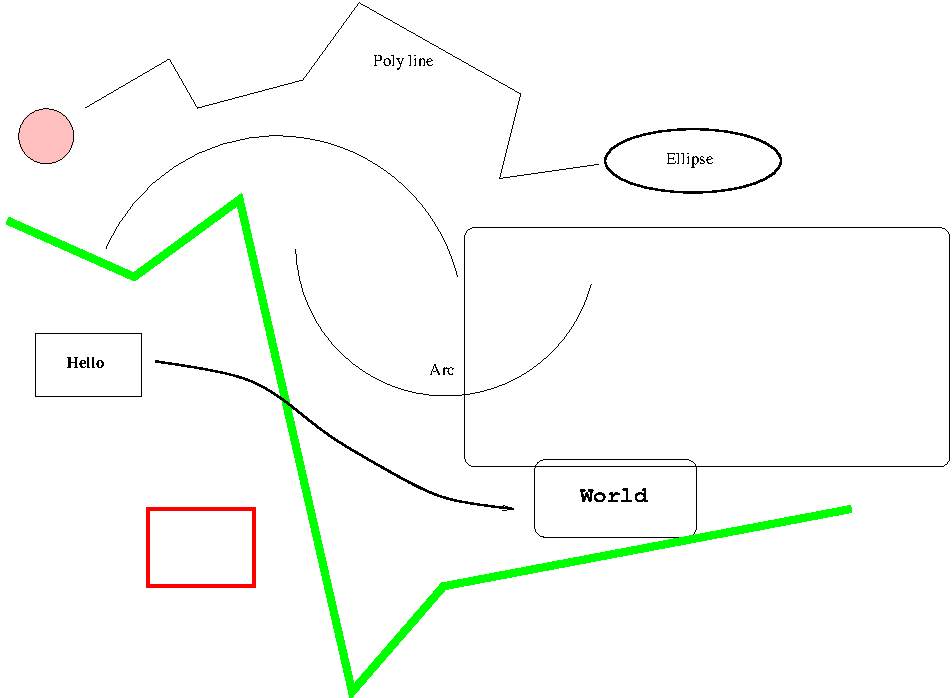
\includegraphics{figs/diagram.pdf}}
\caption{Example diagram drawn using \texttt{xfig}}
\label{xfig}
\end{figure}


\chapter{Evaluation}

\section{Printing and binding}

Use a ``duplex'' laser printer that can print on both sides to print
two copies of your dissertation. Then bind them, for example using the
comb binder in the Computer Laboratory Library.

\section{Further information}

See the Unix Tools notes at

\url{http://www.cl.cam.ac.uk/teaching/current-1/UnixTools/materials.html}


\chapter{Conclusion}

I hope that this rough guide to writing a dissertation is \LaTeX\ has
been helpful and saved you time.


%%%%%%%%%%%%%%%%%%%%%%%%%%%%%%%%%%%%%%%%%%%%%%%%%%%%%%%%%%%%%%%%%%%%%
% the bibliography
\addcontentsline{toc}{chapter}{Bibliography}
\bibliography{refs}

%%%%%%%%%%%%%%%%%%%%%%%%%%%%%%%%%%%%%%%%%%%%%%%%%%%%%%%%%%%%%%%%%%%%%
% the appendices
\appendix

\chapter{Latex source}

\section{diss.tex}
{\scriptsize\verbatiminput{diss.tex}}

\section{proposal.tex}
{\scriptsize\verbatiminput{proposal.tex}}

\chapter{Makefile}

\section{makefile}\label{makefile}
{\scriptsize\verbatiminput{makefile.txt}}

\section{refs.bib}
{\scriptsize\verbatiminput{refs.bib}}


\chapter{Project Proposal}

% Note: this file can be compiled on its own, but is also included by
% diss.tex (using the docmute.sty package to ignore the preamble)
\documentclass[12pt,a4paper,twoside]{article}
\usepackage[pdfborder={0 0 0}]{hyperref}
\usepackage[margin=25mm]{geometry}
\usepackage{graphicx}
\usepackage{parskip}
\begin{document}

\begin{center}
\Large
Computer Science Tripos -- Part II -- Project Proposal\\[4mm]
\LARGE
Conflict Free Document Editing with Different Technologies\\[4mm]

\large
J.~Send, Trinity Hall

Originator: J.~Send

10 October 2016
\end{center}

\vspace{5mm}

\textbf{Project Supervisor:} S.~Kollmann

\textbf{Director of Studies:} Prof.~S.~Moore

\textbf{Project Overseers:} Prof.~T.~Griffin \& Prof.~P.~Lio

% Main document

\section*{Introduction}

\subsection*{Background}

In a world of ever increasing connectivity, collaborative features of applications
will take on greater and greater roles. Popular services such as Google Docs offer real-time
editing of documents by multiple users, a type of interaction that will move from being
a special offering by few applications to a common and expected interface.

The key property that must be implemented to achieve concurrent editing is eventual consistency,
meaning that all connected users should end up with the same result after receiving all changes to the document 
(even if edits conflict). There are two main technologies that are used to enable concurrent editing of a 
document (plain text or otherwise). One approach is Operational Transforms (OT), 
which that generally relies  on having a central server receive, serialize, transform, and 
relay edits occurring simultaneously to each client. OT is notoriously difficult to implement 
correctly as incoming operations have to be transformed against preceding ones on each client, 
such that the result converges. The server may also be required to make some transformations. 
Due to this, central server must be able to read all the operations being performed by clients.
Thus, unless the server is trusted and secure, OT-based services cannot provide any security or privacy guarantees. 

The alternative, newer technology uses Conflict Free Replicated Datatypes (CRDTs). Instead of resolving conflicts and guaranteeing
eventual consistency by transforming operations against each other, CRDTs use special datastructures that guarantee
that no operations will conflict. There are many types of CRDTs that are tailored for different situations. One example
is a simple up-down counter which could be implemented as two locally replicated registers, one for increments and one
for decrements, where the current state is their difference. Compared to OT, there is no interdependence between edits (as long
as the network protocol can guarantee in-order delivery), which means CRDT-based systems can do away with the server
and be implemented using peer to peer (P2P) protocols. This lends itself to security (encryption is now possible between endpoints),
and possibly more scalability and efficiency.

This project is first concerned with exploring and developing a P2P CRDT concurrent text editor, and secondly comparing it to
the OT-based client/server approach available in the open source library ShareJS. Several extensions are also possible,
listed in later sections.

\subsection*{Resources required}

The primary external resource I will need is the library ShareJS, which is published under the MIT license on GitHub.

Additionally, I will be developing on my personal computer, a Thinkpad T440s with 8 GiB of RAM,
128 GB of hard drive space, and a low wattage dual core Intel CPU running at 1.60GHz.
The primary development environment will be under Ubuntu Linux, though Windows 10 is also available 
on the same machine. 

Git with Github will be used as both a version control system and a cloud backup. Dropbox will 
provide continuous cloud backups as well. Backup development machines are any of the MCS computers.

\subsection*{Starting point}

I have some knowledge of the open source library ShareJS from a past internship, which I aim to leverage when 
evaluating and comparing it to my system. My knowledge of CRDTs and the relevant adding/insert/merge
algorithms stems mostly from a high level explanation provided by Martin Kleppmann, along with a diagram.
This will be the starting point for my from-scratch implementation of the concurrent text editor.

Since I have no experience writing test cases and performance profiling, nor network simulation, 
I will have to learn how to do these.

Lastly, I may consult various papers on CRDTs, as well as my supervisor's work in the area, if required.

\section*{Work to be done}

\subsection*{Overview}
I plan to implement a simulation of P2P CRDT text editing using Javascript. Following this, my project will focus on
comparing an existing OT-based concurrent document editing library (ShareJS) to my implementation, in order to draw conclusions
about their relative network and memory efficiency, and scalability. It is highly likely that my 
system will need some optimization, which can feed back into my evaluation and comparison process. In the case that
these phases do not take too long, there are several possible extensions. The first would be to add
a networking layer to the simulation - in effect turning the it into a usable library. The second would be
researching and implementing 'undo' and 'move' operations, which are relatively open research problems.

\subsection*{Detailed Project Structure}

\begin{enumerate}

\item \textbf{Proposal:} Done.

\item \textbf{Core CRDT Development:} Consider and decide on CRDT datastructure. Then detail how I expect
the insert/delete/merge algorithms to work on paper, followed by implementing these. Lastly, I will need to
learn frameworks for testing my implementation. Both hand-coded and automated tests for correctness should be included.

\item \textbf{Implement Simulation:} Model having an arbitrary number of clients each running the CRDT algorithms, and simulate
networking between these clients. Because this is P2P, it may be worth adding functionality for a variety of network
topologies.

\item \textbf{Set up ShareJS and Compare:} Set up the ShareJS environment, mirror functionality and setups 
between two systems as much as possible, and create corresponding performance profiling tests for both 
systems. These will focus on network efficiency, memory usage, and scalability.

\item \textbf{Tune Implementation:} There will likely be opportunity for some optimization, which will
feed back into the performance comparisons in the previous step and help evaluate the optimizations themselves.

\item \textbf{Extensions:} The first extension would be to implement a proper P2P network stack and remove the simulated 
networking. Next would be to research undo and move operations and perhaps try to implement one or both of these.

\end{enumerate}



\subsection*{Possible extensions}

There are two extensions of varying difficulty:

\begin{itemize}

\item (Easier) Replace networking simulation with a P2P networking library. The end result of this extension should be a ready to deploy Javascript library.

\item (Difficult) Research prior work on undo and move functionality using CRDTs. If something suitable is found, implement it. Otherwise, attempt to work toward my own solution.

\end{itemize}


\section*{Success criteria}

These are the main success criteria associated with my project

\begin{enumerate}
\item A concurrent text editor based on CRDTs has been implemented.

\item The concurrent text editor passes all correctness tests.

\item Quantitative results comparing ShareJS and the CRDT based system have been obtained and analyzed.
\end{enumerate}


\section*{Timetable}

Planned starting date is 16/10/2011.

\begin{enumerate}

\item \textbf{Michaelmas weeks 2--3} Develop CRDT datastructure and algorithms on paper. Read into P2P networks 
and simulating them.

\item \textbf{Michaelmas weeks 4--5} Lay out project files and implement network simulation with support for different
P2P topologies.

\item \textbf{Michaelmas weeks 6--8} Implement CRDT datastructures and algorithms, and connect these to network simulation.

\item \textbf{Michaelmas vacation} Learn an appropriate testing framework, write and generate unit tests for correctness of implementation. Fix any bugs discovered by the testing process. Set up ShareJS environment. Begin outlining progress report.

\item \textbf{Lent weeks 0--1} Complete progress report. Mirror functionality of ShareJS to the setup
of my system. Start writing performance benchmarks and scalability tests for both systems.

\item \textbf{Lent weeks 2--4} Execute tests and analyze results. Try to explain differences and similarities observed.
Tune my implementation and evaluate various optimizations. Begin writing dissertation. 

\item \textbf{Lent weeks 5--6} Continue writing dissertation and optimizing system. Begin research for extension
which implements proper networking stack.

\item \textbf{Lent weeks 7--8} Continue writing dissertation. Before terms ends, review and peer-review (including supervisor)
incomplete draft. Implement networking extension. Research undo and move operations with CRDTs.

\item \textbf{Easter vacation:} Finish dissertation draft. Work on undo and move extensions for system.

\item \textbf{Easter term 0--2:} Edit and proof read dissertation. Work on extensions.

\item \textbf{Easter term 3:} Proof read and then submit early to concentrate on exams.

\end{enumerate}


\end{document}


\end{document}
